

\section{Experimental Results and Discussion}

Because we can either update pre-trained word embeddings during training or not, through the evaluation, we want to answer the following questions:
\begin{itemize}
\item How well do different word embeddings perform in all tasks when supervised fine-tuning is \textit{not} performed?
\item How well do different word embeddings perform in all tasks when supervised fine-tuning is performed?
\item How does the size of labeled training data affect the experimental results?
\item How well do the word embeddings perform for unknown words? 
\item How do the key parameters of each word learning algorithms affect the experimental results?
\end{itemize}


\begin{table}
\begin{small}
\begin{tabular}{lll}
\hline
%\caption{Benchmark results vs. our best results}
\textbf{Task} & \textbf{Benchmark} & \textbf{Us} \\ \hline
POS-Tagging & (Accuracy) 97.24 \cite{•} & \\  % Toutanova et al. (2003)
Chunking & (F1) 94.29 \cite{•} & \\  % Sha and Pereira (2003)
NER & (F1) 89.31 \cite{•} & \\  % Ando and Zhang (2005)
MWE & (F1) 57.71 \cite{•} & \\  % Schneider (2014), Table 3 exact match on test set
\hline
\label{benchmark}
\end{tabular}
\end{small}
\end{table}



%%%%%%%%%%%%%%%%%%%%%%%%%%%%
%%% BESTS
\begin{figure*}
\caption{Best results for each method for POS-Tagging and Chunking}
\centering
\begin{subfigure}{.5\textwidth}
	\centering
    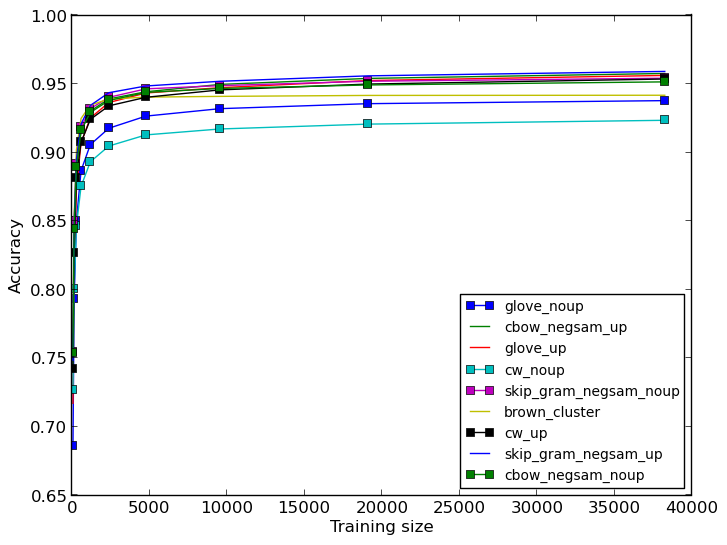
\includegraphics[width=0.8\textwidth]{plots/bestPOS.png}    	
	\label{fig:bestpos}
	\subcaption{POS-Tagging results}	
\end{subfigure}%
\begin{subfigure}{.5\textwidth}
	\centering
    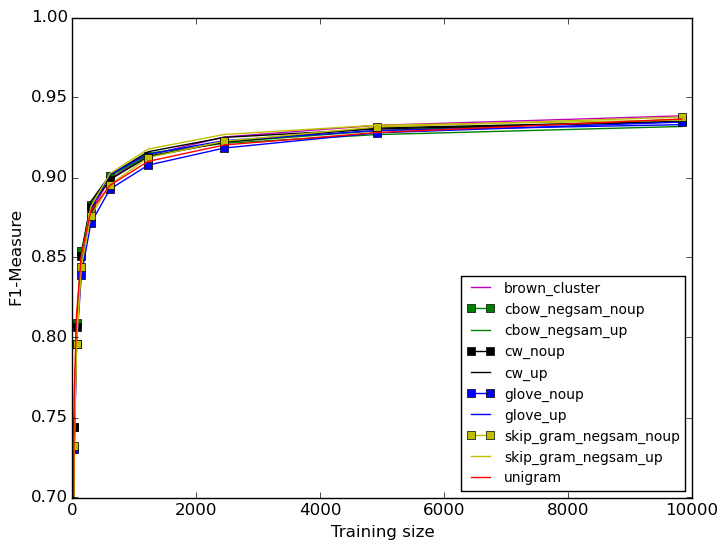
\includegraphics[width=0.8\textwidth]{plots/bestChunking.png}
	\label{fig:bestchunking}
	\subcaption{Chunking results}	
\end{subfigure}
\end{figure*}

\begin{figure*}
\caption{Best results for each method for NER and MWE}
\centering
\begin{subfigure}{.5\textwidth}
	\centering
    	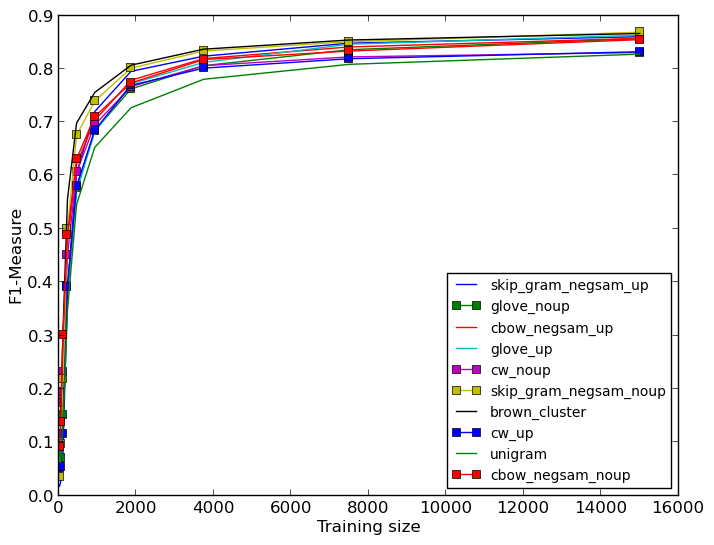
\includegraphics[width=0.8\textwidth]{plots/bestNER.png}
	\subcaption{NER results}	
	\label{fig:bestner}
\end{subfigure}
\begin{subfigure}{.5\textwidth}
	\centering
    	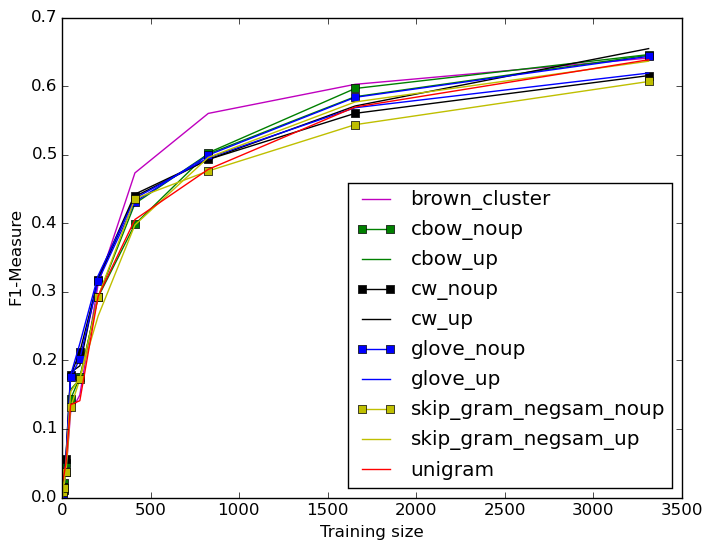
\includegraphics[width=0.8\textwidth]{plots/bestMWE.png}
    \subcaption{MWE results}	
	\label{fig:bestmwe}
\end{subfigure}  	
\end{figure*}  	


%%%%%%%%%%%%%%%%%%%%%%%%%%%%
%%% OUT OF VOC POS

\begin{figure*}
\caption{POS-Tagging out-of-vocabulary-words accuracy for \textit{in-domain} and \textit{out-of-domain} test sets}
\centering
\begin{subfigure}{.5\textwidth}
	\centering
    	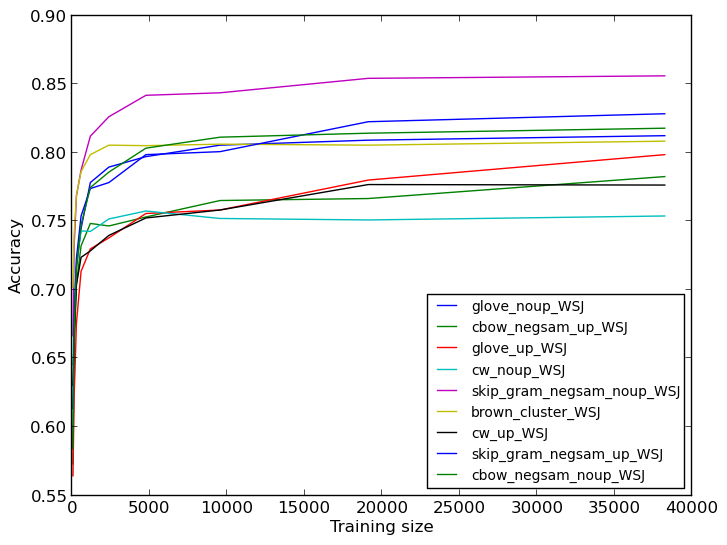
\includegraphics[width=0.8\textwidth]{plots/POSoutOfVocIN.png}
    	\subcaption{\textit{in domain} }
	\label{fig:inpos}
\end{subfigure}
\begin{subfigure}{.5\textwidth}
	\centering
    	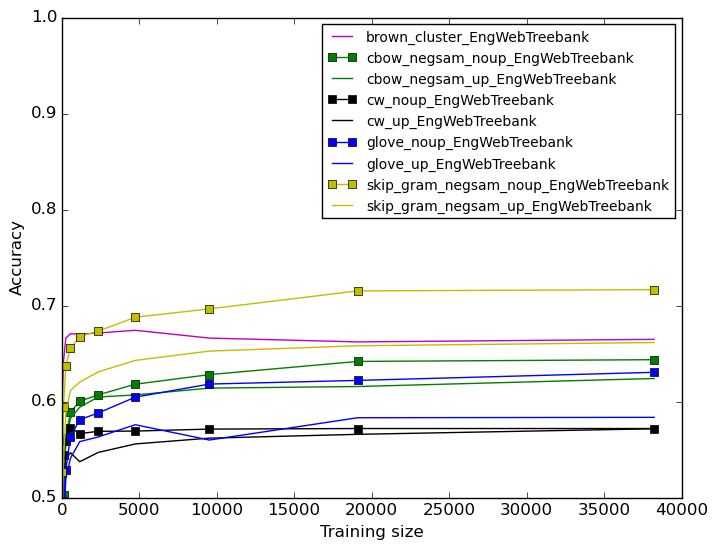
\includegraphics[width=0.8\textwidth]{plots/POSoutOfVocOUT.png}
   	\subcaption{\textit{out-of-domain}}
	\label{fig:outpos}
\end{subfigure}  	
\end{figure*} 

%%%%%%%%%%%%%%%%%%%%%%%%%%%%
%%% OUT OF VOC Chunking: missing result!!!

%%%%%%%%%%%%%%%%%%%%%%%%%%%%
%%% OUT OF VOC NER
\begin{figure*}
\caption{NER out-of-vocabulary-words accuracy for \textit{in-domain} and \textit{out-of-domain} test sets}
\centering
\begin{subfigure}{.5\textwidth}
	\centering
    	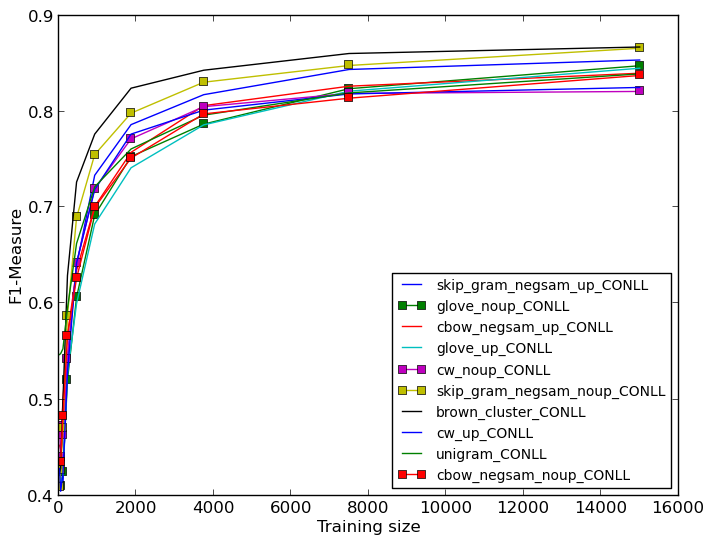
\includegraphics[width=0.8\textwidth]{plots/NERoutOfVocIN.png}
    	\subcaption{\textit{in-domain}}
	\label{fig:inner}
\end{subfigure}
\begin{subfigure}{.5\textwidth}
	\centering
    	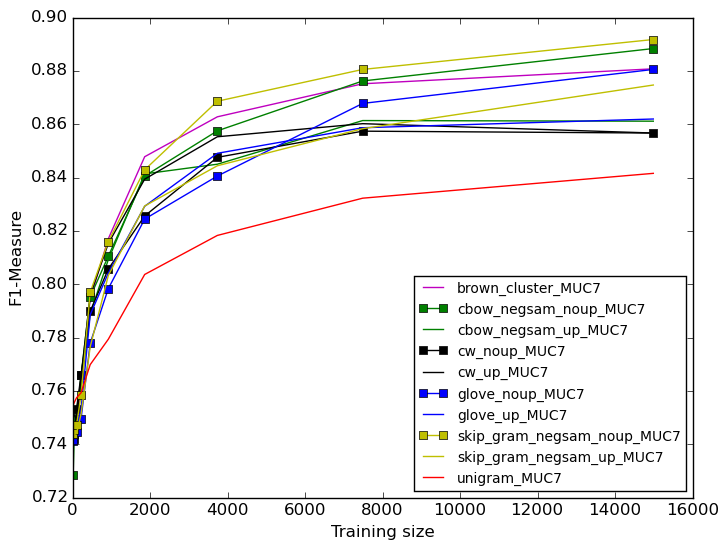
\includegraphics[width=0.8\textwidth]{plots/NERoutOfVocOUT.png}
   	\subcaption{\textit{out-of-domain}}
	\label{fig:outner}
\end{subfigure}  	
\end{figure*}


%%%%%%%%%%%%%%%%%%%%%%%%%%%%
%%% OUT OF VOC MWE
\begin{figure*}
\caption{MWE out-of-vocabulary-words accuracy for \textit{in-domain} test set}
\centering
    	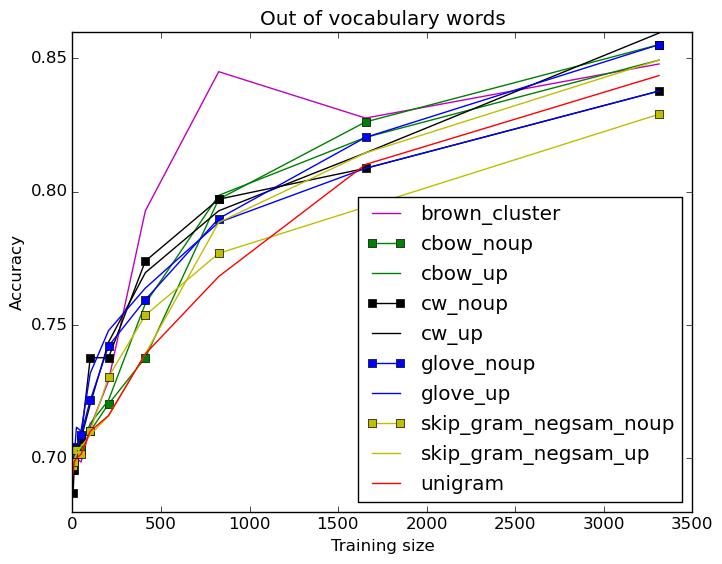
\includegraphics[width=0.5\textwidth]{plots/MWEoutOfVoc.png}    
\label{fig:outmwe}
\end{figure*}

%%%%%%%%%%%%%%%%%%%%%%%%%%%%
%%% OUT OF VOC POS

\subsection{Result tables}

The first column of each table contains the number of training sentences.

\subsubsection{Best hyperparameters for All Tasks}

\begin{table*}[h]
\centering
\begin{adjustbox}{max width=\textwidth}
\pgfplotstabletypeset[col sep=comma, 
precision=4,
every head row/.style={
before row=\toprule,
after row=\midrule},
every last row/.style={
after row=\bottomrule
}]{eval_results/key_results/POS/Accuracy.csv}
\end{adjustbox}
\caption{Accuracy of POS tagging evaluated on WSJ test set}
\label{table:accuracy_pos}
\end{table*}

\begin{table*}[h]
\centering
\begin{adjustbox}{max width=\textwidth}
\pgfplotstabletypeset[col sep=comma, 
precision=4,
every head row/.style={
before row=\toprule,
after row=\midrule},
every last row/.style={
after row=\bottomrule
}]{eval_results/key_results/NER/CONLL_F1Measure.csv}
\end{adjustbox}
\caption{F1 Measure of NER evaluated on CoNLL test set}
\label{table:f1_ner}
\end{table*}

\begin{table*}[h]
\centering
\begin{adjustbox}{max width=\textwidth}
\pgfplotstabletypeset[col sep=comma, 
precision=4,
every head row/.style={
before row=\toprule,
after row=\midrule},
every last row/.style={
after row=\bottomrule
}]{eval_results/key_results/chunking/chunks_F1Measure.csv}
\end{adjustbox}
\caption{F1 Measure of chunking evaluated on CoNLL test set}
\label{table:f1_chunking}
\end{table*}

\begin{table*}[h]
\centering
\begin{adjustbox}{max width=\textwidth}
\pgfplotstabletypeset[col sep=comma, 
precision=4,
every head row/.style={
before row=\toprule,
after row=\midrule},
every last row/.style={
after row=\bottomrule
}]{eval_results/key_results/MWEs/mwe_F1Measure.csv}
\end{adjustbox}
\caption{F1 Measure of MWE identification evaluated on MWE test set}
\label{table:f1_mwe}
\end{table*}

\subsubsection{Out of Vocabulary results for All Tasks}

\begin{table*}[h]
\centering
\begin{adjustbox}{max width=\textwidth}
\pgfplotstabletypeset[col sep=comma, 
precision=4,
every head row/.style={
before row=\toprule,
after row=\midrule},
every last row/.style={
after row=\bottomrule
}]{eval_results/key_results/POS/WSJ_out-of-vocabulary_Accuracy.csv}
\end{adjustbox}
\caption{Accuracy of POS tagging evaluated on out-of-vocabulary words in WSJ test set}
\label{table:outVocab_pos_accuracy}
\end{table*}

\begin{table*}[h]
\centering
\begin{adjustbox}{max width=\textwidth}
\pgfplotstabletypeset[col sep=comma, 
precision=4,
every head row/.style={
before row=\toprule,
after row=\midrule},
every last row/.style={
after row=\bottomrule
}]{eval_results/key_results/NER/CONLL_out-of-vocabulary_Accuracy.csv}
\end{adjustbox}
\caption{Accuracy of NER evaluated on out-of-vocabulary words in CoNLL test set}
\label{table:outVocab_ner_accuracy}
\end{table*}

\begin{table*}[h]
\centering
\begin{adjustbox}{max width=\textwidth}
\pgfplotstabletypeset[col sep=comma, 
precision=4,
every head row/.style={
before row=\toprule,
after row=\midrule},
every last row/.style={
after row=\bottomrule
}]{eval_results/key_results/chunking/Accuracy.csv}
\end{adjustbox}
\caption{Accuracy of Chunking evaluated on out-of-vocabulary words in CoNLL test set}
\label{table:outVocab_chunking_accuracy}
\end{table*}

\begin{table*}[h]
\centering
\begin{adjustbox}{max width=\textwidth}
\pgfplotstabletypeset[col sep=comma, 
precision=4,
every head row/.style={
before row=\toprule,
after row=\midrule},
every last row/.style={
after row=\bottomrule
}]{eval_results/key_results/MWEs/out-of-vocabulary_Accuracy.csv}
\end{adjustbox}
\caption{Accuracy of MWE identification evaluated on out-of-vocabulary words in MWE test set}
\label{table:outVocab_mwe_accuracy}
\end{table*}

\subsubsection{Out of domain Results for NER and POS}

\begin{table*}[h]
\centering
\begin{adjustbox}{max width=\textwidth}
\pgfplotstabletypeset[col sep=comma, 
precision=4,
every head row/.style={
before row=\toprule,
after row=\midrule},
every last row/.style={
after row=\bottomrule
}]{eval_results/key_results/POS/EngWebTreebank_Accuracy.csv}
\end{adjustbox}
\caption{Accuracy of POS tagging evaluated on English web treebank.}
\label{table:outDomain_accuracy_pos}
\end{table*}

\begin{table*}[h]
\centering
\begin{adjustbox}{max width=\textwidth}
\pgfplotstabletypeset[
col sep=comma, 
precision=4,
every head row/.style={
before row=\toprule,
after row=\midrule},
every last row/.style={
after row=\bottomrule
}]{eval_results/key_results/NER/MUC7_chunks_F1Measure.csv}
\end{adjustbox}
\caption{F1 measure of NER evaluated on MUC7 test set}
\label{table:outDomain_ner_f1}
\end{table*}


\section{Conclusion}
